% !TEX root = ../../prj4projektdokumentation.tex

\section{Belastning}
\subsection{Beregning for Belastning}
Med denne distributionslinje og med trinskifteren, der står på 4V trinnet, kan det beregnes hvilken belastning, der vil medføre, at spændingen hos forbrugeren falder til under 10 \% \\ af 4V. Kredsløbet og beregningen ses nedenfor.

\begin{figure}[htbp] % (alternativt [H])
	\centering
	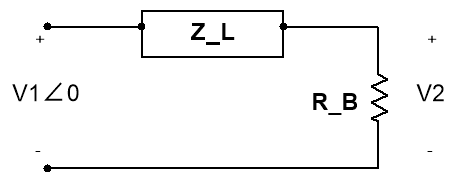
\includegraphics[width=0.4\textwidth]{Figure/Belastningberegning}
	\caption{Kredsløb til beregning af belastning}
	\label{fig:Belastningberegning}
\end{figure}

Først bruges spændingsdelerformlen

\begin{align}
	V2=V1\cdot\frac{R_B}{Z_L+R_B}
\end{align}

\begin{align}
	0,9\cdot\vert V1 \vert = \vert V1\cdot\frac{R_B}{Z_L+R_B} \vert = V1\cdot\frac{R_B}{R_L+jX_L+R_B}
\end{align}

\begin{align}
0,9= \vert \frac{R_B}{R_L+jX_L+R_B} \vert
\end{align}

\begin{align}
	0,9\cdot\vert R_L+jX_L+R_B \vert = \vert R_B \vert
\end{align}

\begin{align}
0,9\cdot\sqrt{(R_L+R_B)^2+X_L^2}=R_B
\end{align}

\begin{align}
(R_L+R_B)^2+X_L^2=\frac{R_B^2}{0,81}
\end{align}

\begin{align}
R_L^2+R_B^2+2\cdot R_L\cdot R_B+X_L^2=\frac{R_B^2}{0,81}
\end{align}

\begin{align}
R_B^2\cdot (1-\frac{1}{0,81})+2\cdot R_L\cdot R_B+X_L^2=0
\end{align}

Værdier indsættes og herved fås:

\begin{align}
R_B^2\cdot (-0,24) +12,4\Omega\cdot R_B+18,23\Omega=0
\end{align}

Andengrads ligning løses og derved findes den modstandsværdi, der vil give et spændingsfald på 10\%.

\begin{align}
R_B=\frac{-12,4\pm\sqrt{153,76-4\cdot(-0,24)\cdot18,23}}{-0,24\cdot 2}=\frac{-12,4\pm 13,1}{-0,47}=54,3 \Omega
\end{align}

Denne modstandsværdi i det viste kredsløb og med den valgte distributionslinje vil resultere i at spændingen falder under det ønskede niveau som er 4V. Der tages derfor udgangspunkt i denne værdi, men efterfølgende vil belastninger bestemmes ud fra simuleringer i værktøjet Multisim. Simulering der understøtter beregningerne ses på figur \ref{fig:powfacsim}

\subsection{Implementering af Belastning}
\label{subsec:implementeringAfBelastning}
Til implementering af belastninger/forbrugere er der på baggrund af foregående beregninger valgt modstande i intervallet 16 $\Omega$ til 100 $\Omega$. Belastninger er placeret i parallel og til hver belastning hører en kontakt, således der let kan skiftes mellem forskellige værdier. Der er desuden monteret pin til forbindelse til distributionslinje og bananstik til forbindelse til 0V på transformeren. Yderligere er der for hver belastning monteret en 1 $\Omega$ modstand således Måleenheden kan overvåge tilstanden hos hver forbruger. Det færdige print med belastninger ses på figur \ref{fig:Belastning1}

\begin{figure}[H] 
	\centering
	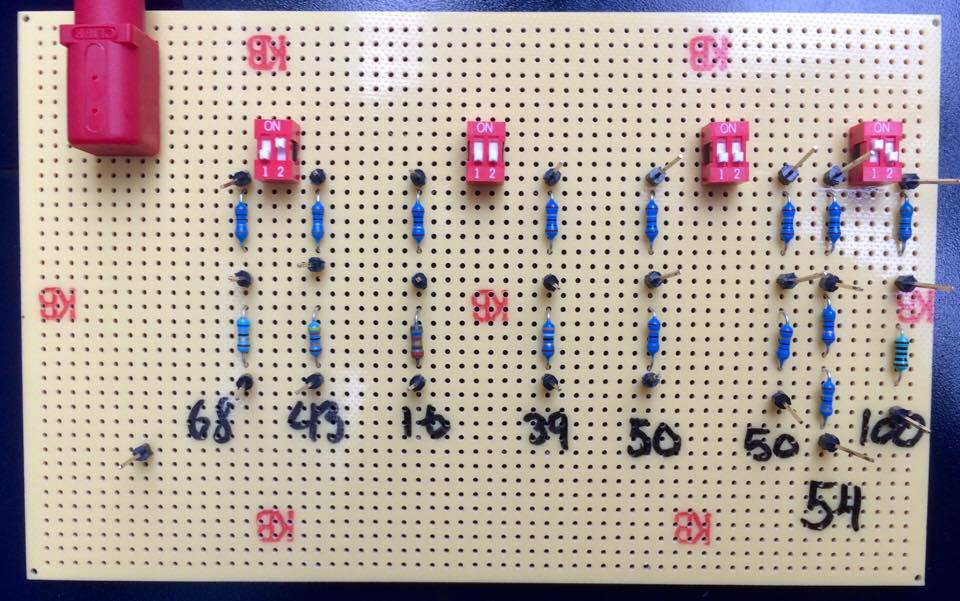
\includegraphics[width=0.7\textwidth]{Figure/Belastningskreds}
	\caption{Færdigt print med belastninger/forbrugere}
	\label{fig:Belastning1}
\end{figure}


\section{Power factor}

For yderligere monitorering ønskes det også at undersøge power factor i systemet. Når effekt transporteres gennem en distributionslinje består det af både aktiv og reaktiv effekt, og power factor fortæller ratioen mellem aktiv og tilsyneladende effekt. Denne parameter fortæller hvor meget effekt, der kan tages ud af systemet og udnyttes hos en belastning/forbruger. Da belastningerne i dette system er rent ohmske, og der kun er spolevirkning fra 'kablet, forventes der en power factor tæt på 1, men som vil være lagging netop pga, spolen. Forholdet mellem aktiv, reaktiv og tilsyneladende effekt kan ses på figur \ref{fig:Effekttrekant}

\begin{figure}[H] 
	\centering
	\includegraphics[width=0.5\textwidth]{Figure/Effekttrekant}
	\caption{Effekttrekant}
	\label{fig:Effekttrekant}
\end{figure}

På baggrund af dette kan den aktuelle power factor med de valgte kabelparametre og en belastning på 54 $\Omega$ nu beregnes. Beregninger ses nedenfor.

\begin{align}
Z_R=54 \Omega
\end{align}
\begin{align}
R_L=6,2\Omega
\end{align}
\begin{align}
X_L=2*\pi*50Hz*13,6mH=4,27\Omega
\end{align}
\begin{align}
Z_D=(6,2+4,27j)\Omega
\end{align}
\begin{align}
Z_L=Z_R+Z_D=(60,2+4,27j)\Omega
\end{align}
\begin{align}
I=\frac{4V}{\vert Z_L \vert} = 0,07 A
\end{align}
\begin{align}
S_L=I^2\cdot Z_L = (0,26+0,02j) VA
\end{align}
\begin{align}
P=0,26 W
\end{align}
\begin{align}
pf= \frac{P}{\vert S_L \vert} = 0,996
\end{align}

For at tjekke og understøtte disse beregninger er der lavet en simulering af systemet i Multisim. Denne simulering giver en power factor på 0,997, hvilket stemmer fint overens med forventningen fra beregningen. Simuleringen ses på figur \ref{fig:powfacsim} 

\begin{figure}[H] 
	\centering
	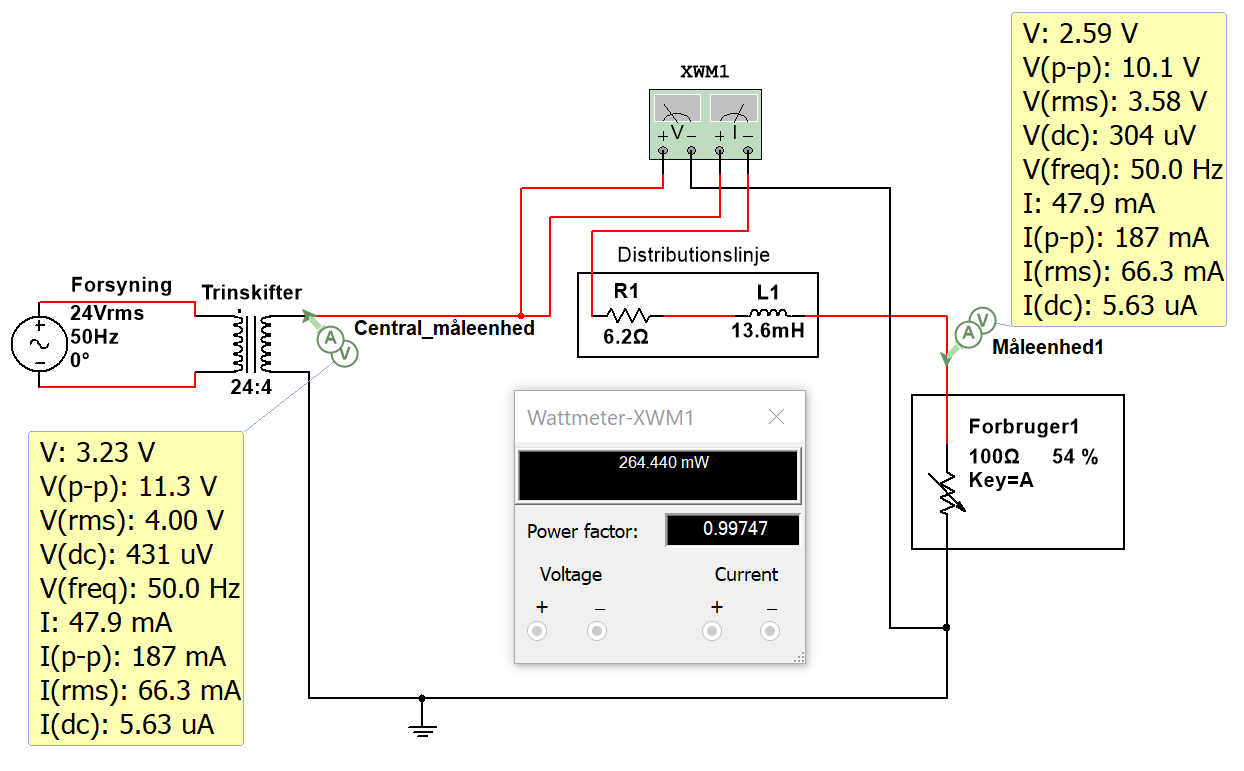
\includegraphics[width=1\textwidth]{Figure/powerfactormultisim}
	\caption{Simulering, der viser power factor}
	\label{fig:powfacsim}
\end{figure}